\documentclass[a4paper,12pt]{article}

\usepackage[utf8]{inputenc}
\usepackage[english, greek]{babel}
\usepackage{geometry}
\usepackage{paralist}
\usepackage{wrapfig}
\usepackage{graphicx}
\usepackage{subcaption} 
\usepackage{hyperref}

\geometry{left=2.5cm,right=2.5cm, top=2cm, bottom=2cm}
\newcommand{\en}{\selectlanguage{english}}
\newcommand{\gr}{\selectlanguage{greek}}
\renewcommand{\arraystretch}{1.5}
\graphicspath{ {./images/} }


\begin{document}
\begin{titlepage}
	\begin{center}
		\vspace*{5cm}
		
		{\LARGE Ενσωματωμένα Συστήματα Πραγματικού Χρόνου} \\		
		\vspace{1cm}
		
		{\Large Εργασία 1} \\
		\vspace{5cm}
		
		\begin{large}
			Σύνδεσμος κώδικα: \href{https://github.com/AlexDelitzas/embedded-systems-course}{\textlatin{Github}} \\
		\end{large}
		\vspace{4cm}
		\begin{large}
			Όνομα : Αλέξανδρος Δελητζάς \\
			ΑΕΜ : 8448 \\
			\en
			e-mail : adelitzas@ece.auth.gr \\
			\gr
		\end{large}
		
		\vfill
		\today
		
	\end{center}
\end{titlepage}


\newpage

\section{Εισαγωγή}
Στα πλαίσια της εργασίας αναπτύχθηκαν δύο προγράμματα με σκοπό να γίνει τακτική δειγματοληψία με όσο το δυνατό μικρότερη απόκλιση από τον πραγματικό χρόνο. Στην πρώτη υλοποίηση γίνεται χρήση της \textlatin{nanosleep()}. Για αυτήν την περίπτωση, εξηγείται η ανάγκη για χρήση των \textlatin{timestamps} που συλλέγονται με σκοπό τη βελτίωση της ακρίβειας του χρόνου δειγματοληψίας. Στη δεύτερη υλοποίηση γίνεται χρήση της \textlatin{setitimer()} και διακοπών (\textlatin{interrupts}). Σε αυτή την περίπτωση, η χρήση των \textlatin{timestamps} που συλλέγονται για βελτίωση δεν είναι απαραίτητη. Για την ανάλυση της στατιστικής συμπεριφοράς, τρέξαμε την καθε υλοποίηση για συνολική διάρκεια $t=7200 \, sec$ και περίοδο δειγματοληψίας $\delta t=0.1 \, sec$. Τέλος, θα εξετάσουμε την κατανάλωση ενέργειας των δύο υλοποιήσεων.

\section{Πρώτη Υλοποίηση}

\subsection{Περιγραφή υλοποίησης}
Σε πρώτη φάση, με σκοπό να ρυθμίσουμε τις παραμέτρους της \textlatin{nanosleep()}, εκφράζουμε το χρονικό διάστημα $\delta t$ σε ακέραια \textlatin{seconds} και \textlatin{nanoseconds}. Ο βασικός πυρήνας του προγράμματος είναι ένας βρόχος επανάληψης, ο οποίος τερματίζει όταν συλλεχθεί ο απαραίτητος αριθμός δειγμάτων. Σε κάθε επανάληψη η διεργασία παραμένει αδρανής για το χρονικό διάστημα που ορίζουμε και μετά καλείται η συνάρτηση \textlatin{timerHandler()} για να συλλέξει το τρέχον \textlatin{timestamp}. Τα \textlatin{timestamps} αποθηκεύονται σε έναν πίνακα. Μόλις περάσει ο συνολικός χρόνος δειγματοληψίας ή η διαδικασία διακοπεί από το χρήστη μέσω \textlatin{Ctrl-C}, τότε αποθηκεύονται σε ένα αρχείο. \\
Σε μια πρώτη απόπειρα, ορίσαμε το χρονικό διάστημα της \textlatin{nanosleep()} ίσο με $\delta t$ σε κάθε επανάληψη. Όμως, παρατηρήθηκε ότι συσσωρευόταν σφάλμα από κάθε επανάληψη, με αποτέλεσμα καθώς αυξάνονται οι επαναλήψεις να υπάρχει μεγάλη απόκλιση από τον ιδανικό χρόνο και να χάνονται δείγματα. 
\begin{wraptable}{R}{0.4\textwidth}
	\centering
	\begin{tabular}{ ||p{4cm}|c|| }
		\hline
		Μέγιστο \textlatin{(sec)} & 0.108572 \\
		\hline
		Ελάχιστο \textlatin{(sec)} & 0.091453 \\
		\hline
		Μέσος όρος \textlatin{(sec)} & 0.100000 \\
		\hline
		Διάμεσος \textlatin{(sec)} & 0.100000 \\
		\hline
		Τυπική απόκλιση \textlatin{(sec)} & 0.000078 \\
		\hline
	\end{tabular}
	\caption{Στατιστικά στοιχεία της χρονικής απόστασης μεταξύ δύο διαδοχικών δειγμάτων}\label{tab:stats1}
\end{wraptable}

Για να βελτιώσουμε την ακρίβεια των χρονικών στιγμών δειγματοληψίας, χρησιμοποιήσαμε τα \textlatin{timestamps} που συλλέγουμε. Έτσι, κάθε φορά που καλείται η \textlatin{timerHandler()} προσαρμόζει το επόμενο χρονικό διάστημα της \textlatin{nanosleep()} με τον εξής τρόπο: 
$${\delta t}_{next} =  \delta t - dif, \qquad dif = t_{real} - t_{ideal}$$
όπου $dif$ είναι η διαφορά του \textlatin{timestamp} που συλλέξαμε από το ιδανικό. Στην πραγματικότητα αντί για $dif$ στην υλοποίηση μας, παίρνουμε το \textlatin{floating-point} υπόλοιπο της διαίρεσης $dif/{\delta t}$ ώστε σε περίπτωση που χαθεί κάποιο \textlatin{timestamp} να μην επηρεαστεί ο χρόνος που θα ληφθεί το επόμενο.

\subsection{Στατιστική συμπεριφορά}

Από το πείραμα που έγινε, τα στατιστικά στοιχεία της χρονικής απόστασης μεταξύ δύο διαδοχικών δειγμάτων φαίνονται στον Πίνακα~\ref{tab:stats1}. Αρχικά, ο αριθμός των δειγμάτων που λάβαμε είναι σωστός (το τελευταίο δείγμα λήφθηκε τη χρονική στιγμή $t = 7200.000077 \, sec$). Όπως βλέπουμε, ο μέσος όρος και η διάμεσος είναι ίσες με το $\delta t = 0.1$ που χρησιμοποιήσαμε το οποίο είναι επιθυμητό στοιχείο. Η τυπική απόκλιση είναι της τάξεως των $10^{-5} \, sec$. Από τα στοιχεία αυτά συμπεραίνουμε ότι οι χρονικές αποστάσεις μεταξύ διαδοχικών δειγμάτων δεν απομακρύνονται πολύ από το $\delta t = 0.1$. \\
Στο Σχήμα~\ref{fig:hist1} βλέπουμε την κατανομή των χρονικών αποστάσεων μεταξύ δύο διαδοχικών δειγμάτων. Όπως περιμέναμε, η πλειοψηφία των χρονικών αποστάσεων λαμβάνουν τιμές πολύ κοντά στο $\delta t = 0.1$. Έπειτα όσο απομακρυνόμαστε από το $0.1$ η συχνότητα ακολουθεί μια καθοδική πορεία. Εξαίρεση αποτελούν κάποια μεμονωμένα \textlatin{bins}, στα οποία το γράφημα θα ήταν πιθανότατα πιο εξομαλυμένο αν το πείραμα συνεχιζόταν για περισσότερο από $t = 7200 \, sec$. Το εύρος που βρίσκονται οι μη αμελητέες συχνότητες στην κατανομή είναι $2 \cdot 10^{-4} \, sec$. \\
Στο Σχήμα~\ref{fig:error1} βλέπουμε την απόκλιση των χρονικών στιγμών που λήφθηκαν τα \textlatin{timestamps} από τις ιδανικές. Το σφάλμα αυτό είναι της τάξεως $10^{-4} \, sec$ και σε κάποιες περιπτώσεις λαμβάνει πολύ μικρές τιμές τάξεως $10^{-3} \, sec$.

\begin{figure}
	\hspace{-1cm}
	\begin{subfigure}[b]{0.6\textwidth}
		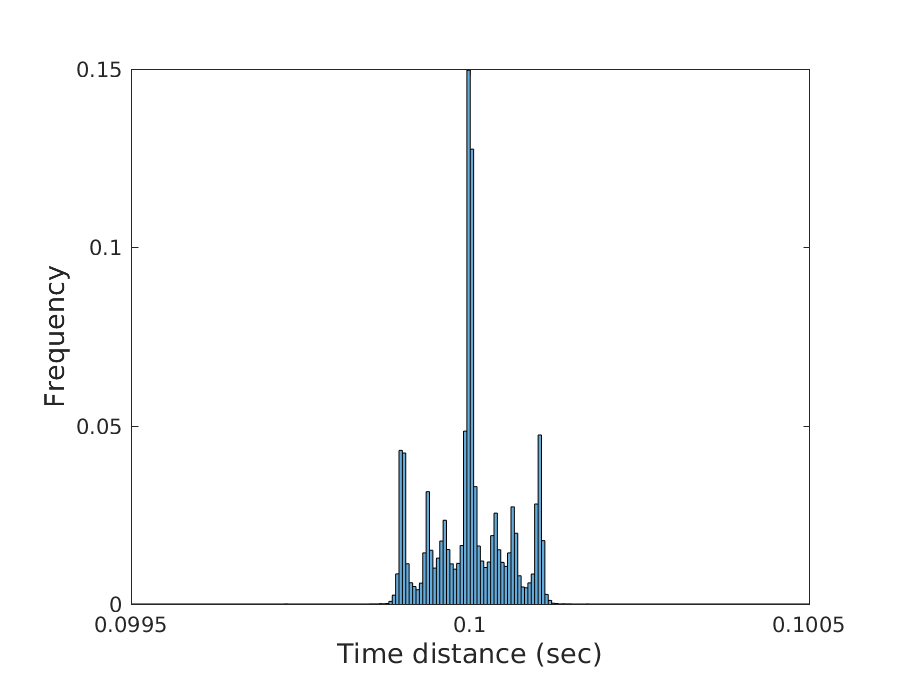
\includegraphics[width=\textwidth]{hist1.eps}
		\caption{Κατανομή των χρονικών αποστάσεων μεταξύ δύο διαδοχικών διεγμάτων}
		\label{fig:hist1}
	\end{subfigure}
	%
	\begin{subfigure}[b]{0.5\textwidth}
		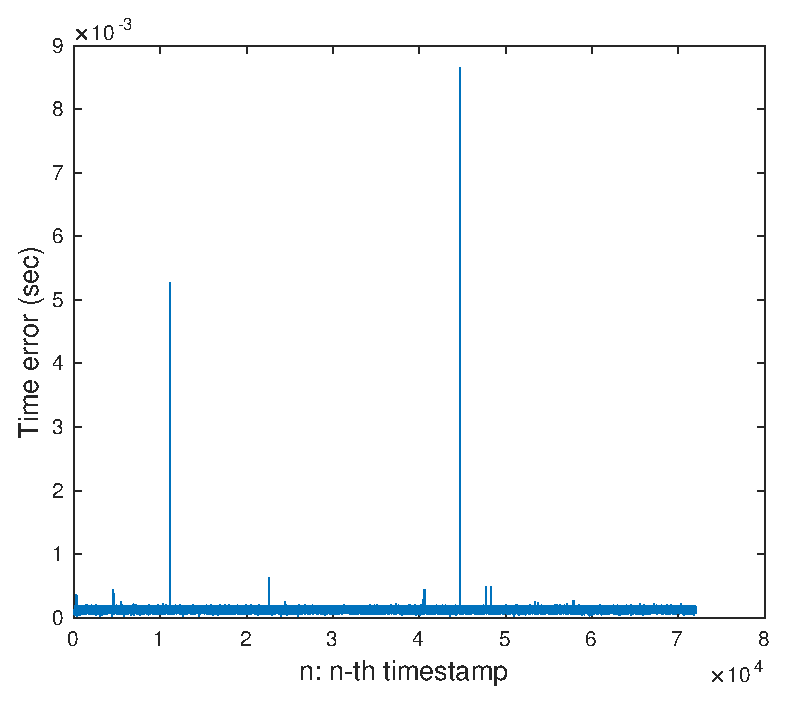
\includegraphics[width=\textwidth]{error1.eps}
		\caption{Απόκλιση των χρονικών στιγμών που λήφθηκαν τα \textlatin{timestamps} από τις ιδανικές}
		\label{fig:error1}
	\end{subfigure}
\end{figure}


\section{Δεύτερη Υλοποίηση} 

\subsection{Περιγραφή υλοποίησης}
Αρχικά, με σκοπό να ρυθμίσουμε τις παραμέτρους της \textlatin{setitimer()}, εκφράζουμε το χρονικό διάστημα $\delta t$ σε ακέραια \textlatin{seconds} και \textlatin{microseconds}. Χρησιμοποιήσαμε την παράμετρο \textlatin{ITIMER\_REAL} της \textlatin{setitimer()}, ώστε να μετρήσουμε σε διαστήματα πραγματικού χρόνου. Έτσι, κάθε φορά που περνάει χρονικό διάστημα $\delta t$ θα σταλεί σήμα \textlatin{SIGALRM} στη διεργασία. \\
Και σε αυτήν την υλοποίηση, ο βασικός πυρήνας του προγράμματος είναι ένας βρόχος επανάληψης, ο οποίος τερματίζει όταν συλλεχθεί ο απαραίτητος αριθμός δειγμάτων. Λόγω της \textlatin{pause()}, σε κάθε επανάληψη η διεργασία παραμένει αδρανής μέχρι να σταλεί το σήμα \textlatin{SIGALRM}. Μόλις συμβεί αυτό, αναλαμβάνει δράση η \textlatin{timerHandler()} (\textlatin{handler} του σήματος \textlatin{SIGALRM}), με σκοπό να συλλέξει το \textlatin{timestamp}.

\subsection{Στατιστική συμπεριφορά}


Από το πείραμα που έγινε, τα στατιστικά στοιχεία της χρονικής απόστασης μεταξύ δύο διαδοχικών δειγμάτων φαίνονται στον Πίνακα~\ref{tab:stats2}. Και πάλι ο αριθμός των δειγμάτων που λάβαμε είναι σωστός (το τελευταίο δείγμα λήφθηκε τη χρονική στιγμή $t = 7200.000019 \, sec$). Όπως και στην προηγούμενη υλοποίηση, ο μέσος όρος και η διάμεσος είναι (σχεδόν) ίσες με το $\delta t = 0.1$. Η τυπική απόκλιση, όμως, λαμβάνει τιμή λίγο μικρότερη. Επίσης, η ελάχιστη και η μέγιστη τιμή βρίσκονται πιο κοντά στο $\delta t = 0.1$, από ότι πριν. \\

\begin{wraptable}{R}{0.35\textwidth}
	\centering
	\begin{tabular}{ ||p{4cm}|c|| }
		\hline
		Μέγιστο \textlatin{(sec)} & 0.103765 \\
		\hline
		Ελάχιστο \textlatin{(sec)} & 0.096236 \\
		\hline
		Μέσος όρος \textlatin{(sec)} & 0.100000 \\
		\hline
		Διάμεσος \textlatin{(sec)} & 0.099999 \\
		\hline
		Τυπική απόκλιση \textlatin{(sec)} & 0.000063 \\
		\hline
	\end{tabular}
	\caption{Στατιστικά στοιχεία της χρονικής απόστασης μεταξύ δύο διαδοχικών δειγμάτων}\label{tab:stats2}
\end{wraptable}
Στο Σχήμα~\ref{fig:hist2} παρατηρούμε ότι και σε αυτή την υλοποίηση η πλειοψηφία των αποστάσεων βρίσκεται γύρω από το $\delta t = 0.1$, όπως είναι το επιθυμητό. Η διαφορά με την προηγούμενη υλοποίηση είναι ότι κάποια μεμονωμένα \textlatin{bins} που χαλούσαν την καθοδική πορεία της κατανομής, καθώς απομακρυνόμαστε από το κέντρο ($\delta t = 0.1$), πλέον έχουν μικρότερη συχνότητα. \\
Όσον αφορά την απόκλιση από τις ιδανικές χρονικές στιγμές δειγματοληψίας (Σχήμα~\ref{fig:error2}) και πάλι είναι της τάξεως $10^{-4}$ με $10^{-3}$ και είναι ελαφρώς μικρότερη από της προηγούμενης υλοποίησης. \\
Συνοπτικά, οι δύο υλοποιήσεις δεν έχουν μεγάλες διαφορές μεταξύ τους. Όμως, η δεύτερη υλοποίηση αποδείχτηκε λίγο πιο αξιόπιστη. 
\begin{figure}[!htbp]
	\hspace{-1cm}
	\begin{subfigure}[b]{0.6\textwidth}
		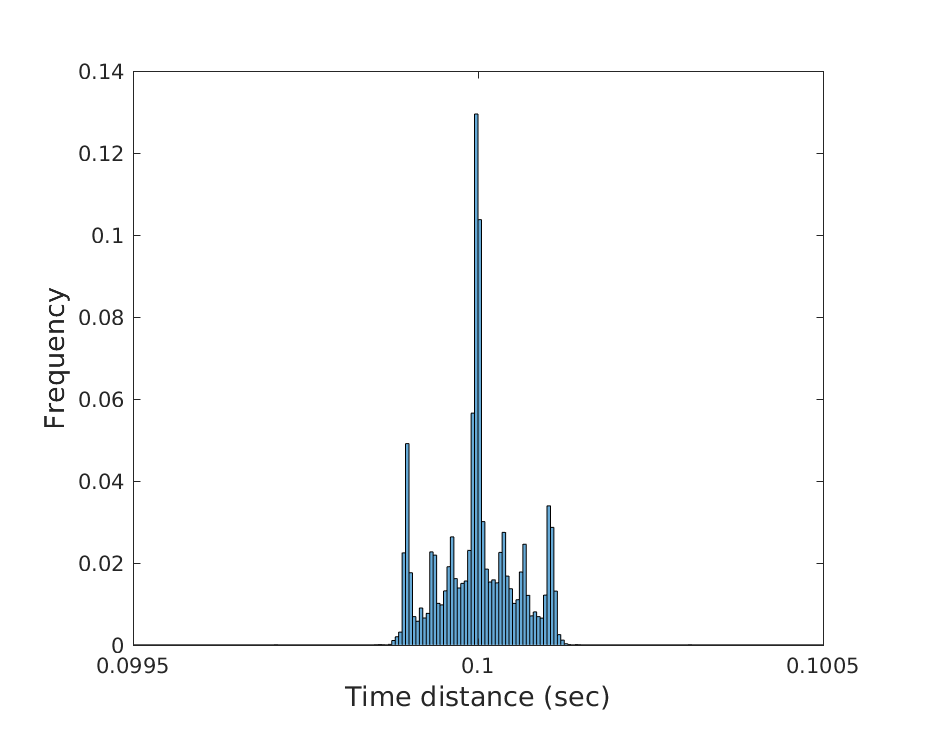
\includegraphics[width=\textwidth]{hist2.eps}
		\caption{Κατανομή των χρονικών αποστάσεων μεταξύ δύο διαδοχικών διεγμάτων}
		\label{fig:hist2}
	\end{subfigure}
	%
	\begin{subfigure}[b]{0.5\textwidth}
		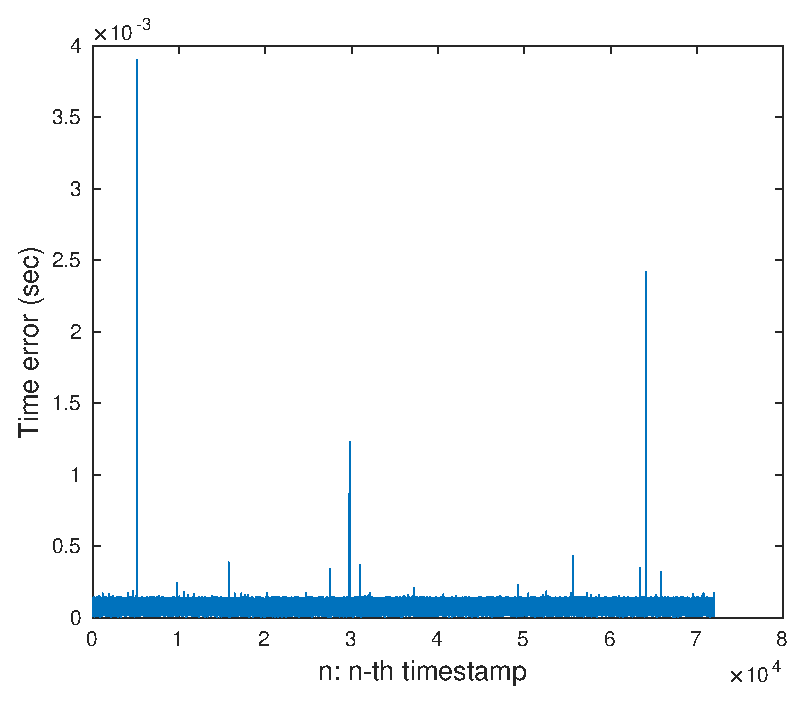
\includegraphics[width=\textwidth]{error2.eps}
		\caption{Απόκλιση των χρονικών στιγμών που λήφθηκαν τα \textlatin{timestamps} από τις ιδανικές}
		\label{fig:error2}
	\end{subfigure}
\end{figure}

\section{Κατανάλωση ενέργειας} 
Όπως αναφέραμε, και στις δύο υλοποιήσεις υπήρξε μέριμνα ώστε:
\begin{inparaitem}
\item η διεργασία να παραμένει αδρανής κατά το χρονικό διάστημα αναμονής,
\item μετά το πέρας του διαστήματος να 'ξυπνάει' για την καταγραφή του \textlatin{timestamp},
\item να επαναλαμβάνεται αυτή η διαδικασία σε όλη τη διάρκεια δειγματοληψίας.
\end{inparaitem}
\\
Με σκοπό την παρακολούθηση της χρήσης της \textlatin{CPU} από τις δύο υλοποιήσεις, δημιουργήσαμε ένα \textlatin{bash script} ( \textlatin{monitor\_cpu.sh} ). Το \textlatin{script} αυτό παίρνει επαναληπτικά μετρήσεις του ποσοστού χρήσης της \textlatin{CPU} που κάνει κάποια διεργασία μέσω της εντολής \textlatin{ps}. Κατά τη διάρκεια των πειραμάτων, θέσαμε την περίοδο μεταξύ των διαδοχικών μετρήσεων υποπολλαπλάσια του $\delta t$ και τρέξαμε το \textlatin{script}. Όπως διαπιστώθηκε, και οι δύο υλοποιήσεις κάναν μηδενική χρήση της \textlatin{CPU}.

\end{document}
